\chapter{GTK+ 移植}{GTK+}

\section{实验目的}
\begin{itemize}
  \item 学习GNU 开源软件的一般移植方法
\end{itemize}

\section{GTK+ 的背景}
GTK+ 是一款跨平台的图形用户接口组件工具包, 原是 GIMP Toolkit 的缩写
(GIMP 是 GNU Image Manipulation Program 的缩写, Linux中重要的图像处理软件,
类似Windows 中的 photoshop), 以GPL版权协议发布, 是 Linux 系统中使用最为
广泛的图形工具之一,许多桌面系统都建立在 GTK+ 基础上, 如著名的 GNOME、xfce4。
(另一个著名的桌面环境 KDE 使用 Qt 库。)

\begin{figure}[h]
  \centering
  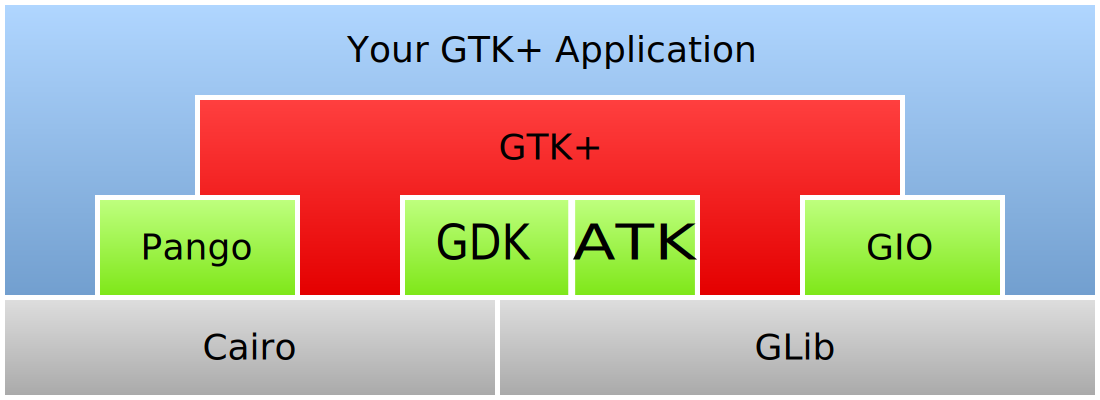
\includegraphics[width=.7\textwidth]{GTK+_architecture}
    \caption[基于GTK+的软件层次结构]
    {基于GTK+的软件层次结构\footnotemark} \label{fig_gtk}
\end{figure}
\footnotetext{图片引自 en.wikipedia.org/wiki}

    GTK+ 不直接和显示硬件设备打交道. Linux 桌面系统通常基于 X-Window. 而在
嵌入式应用中, 作为全功能 X 窗口系统的替代方案, 可以选择DirectFB作为后端. 

\section{GTK+ 库的依赖关系}
从图\ref{fig_gtk}中可以看到, GTK+ 除了为上层应用提供接口函数库以外, 自身也
依赖一系列的更底层的库。图\ref{fig_gtkdfb}是建立 GTK+ 的库依赖关系. 我们
需要根据这样的依赖关系逐层构造系统的API.

\begin{figure}[h]
\centering
\begin{tikzpicture}[level distance=2.5cm, sibling distance=1.2cm,
    nodes={rectangle,minimum width=1.8cm,top color=white,
        bottom color=red!50!black!20,font=\bf},
    level 1/.style={nodes=blue},
    level 2/.style={nodes=red},
    level 3/.style={nodes=green!50!black},
    level 4/.style={nodes=black},
    edge from parent fork right,grow=right,
    edge from parent path={(\tikzparentnode.east) 
        -- (\tikzchildnode.west)}]
\node {gtk+}
    child {node [yshift=-1cm] {atk}
        child {node {glib}
            child {node {dbus}
                child {node {expat}}
            }
            child {node {zlib}}
        }
    }
    child {node {pango}
        child {node {glib}
        }
        child {node {cairo}
            child {node {fontconfig}
                child {node {expat}}
                child {node {freetype}}
                child {node {zlib}}
            }
            child {node {pixman}}
            child {node [yshift=2cm]{DirectFB}
                child {node {libpng}
                    child {node {zlib}}
                }
                child {node {freetype}}
                child {node {libjpeg}}
                child {node {tslib}}
            }
        }
    }
    child {node [yshift=1.5cm] {gdk-pixbuf}
        child {node {libjpeg}}
        child {node {libpng}}
        child {node {glib}}
    }
;
\end{tikzpicture}
  \caption{GTK+的软件依赖关系}\label{fig_gtkdfb}
\end{figure}

本实验中, 我们的最终目标是编译出 gtk+ (建议版本2.22.1) 的库以及演示程序
gtk-demo. 以下根据依赖关系, 对各个库加以简单的说明. 版本号是本实验建议版本.
\begin{itemize}
    \item zlib-1.2.8. zlib 是 Linux 系统最基本的压缩/解压库, 许多软件都会直接
        或间接地用到它. zlib 仅依赖 Glibc. 针对 Linux系统的交叉编译工具链中
        已经包含了 Glibc 的动态和静态库, 编译 zlib 时会自动链接.
        (Linux 系统中几乎所有软件都会链接 Glibc, 下面不再特别说明)

    \item tslib-1.0.0. 触摸屏支持库, 提供人机交互接口的输入支持.
        有关触摸屏库的说明和编译请参考触摸屏移植部分.

    \item libpng-1.2.24. PNG (Portable Network Graphics)是广泛应用于互联网的一种
        图像格式. libpng 依赖 zlib 库的压缩/解压功能.

    \item libjpeg-turbo-1.2.1. JPEG (Joint Photographic Experts Group), 非常
        著名的图像压缩标准格式. libjpeg 是由独立 JPEG 团队 (Independent
        JPEG Group) 开发的处理jpeg图像格式的自由软件. libjpeg-turbo 是
        libjpeg 的一个分支, 它使用 SIMD(Single Instruction Multiple Data)
        指令对 JPEG 的编解码进行加速处理,在x86、ARM、PowerPC
        平台上可以获得比 libjpeg 2到6倍的提速. libjpeg 不依赖其它库.
    \item tiff-3.9.7. 用于处理 TIFF (Tagged Image File Format) 图像格式文件,
        为gdk-pixbuf 提供部分支持, 在本实验中不是必须的.如果编译,
        可依赖 libjpeg,

    \item pixman-0.16.0. 底层像素处理工具 (Pixel Manipulation). 可依赖于
        gtk+, 本实验在编译时禁止该依赖关系.

    \item libxml2-2.6.30/expat-2.0.1. XML (Extensible Markup Language,
        扩展标记语言) 是在互联网中广泛使用的一种标记语言, 既可以让人读懂,
        也能让机器读懂. Linux 系统中的很多软件基于 XML 语言. 目前在Linux
        系统中, 提供 XML 解释功能的主要有两套库: expat 和 libxml2.
        多数软件依赖于 libxml2, 但仍有少数必须依赖 expat. expat 不依赖
        其它软件, libxml2 可以依赖 zlib.

    \item dbus-1.8.16. D-Bus (Desktop BUS) 提供桌面环境下的进程间通信机制,
        属于 freedesktop.org 项目的一部分. dbus 依赖 xml 库, 可选择 libxml
        (不是 libxml2!) 或者 expat. 但由于 libxml 早已停止开发, 所以在编译
        dbus 时指定链接 expat 库.

    \item glib-2.28.8. glib 原始于 GTK+ 计划. 在 gtk+-2版本之前, 不属于
        图形用户接口部分的功能被从 GTK+ 中分离出来单独开发, 这部分就是 glib.
        glib 依赖 dbus 和 zlib.

    \item freetype-2.3.7. freetype 库实现矢量字体TrueType、Type1显示效果支持
        (字体渲染). 在链接 libpng 时还可以支持 png 压缩的点阵字体. freetype
        自身已包含 zlib 解压功能, 可以不依赖 zlib, 也可在编译时指定使用系统的
        zlib.

    \item fontconfig-2.6.0. 字体配置工具, 告诉系统如何找到字体库, 依赖
        freetype、zlib 和 XML. XML 可选择 expat 或者 libxml2.

    \item DirectFB-1.4.1. Direct Frame Buffer 提供图形加速、输入抽象层处理
        以及窗口系统的基本功能, 是 GTK+ 的后端. 它依赖触摸屏库tslib、字体库
        freetype 以及图形库libpng、libjpeg.

        桌面系统的 GTK+ 通常依赖 X-Window, 但 X-Window 涉及的库比较多, 依赖
        关系也比较复杂, 对于小型嵌入式应用来说不如 DirectFB 方便。

    \item cairo-1.8.0. 提供2维矢量图形处理的工具包. 在本实验中, 除后端选择
        DirectFB外, 还依赖 fontconfig、pixman 和 XML.

    \item atk-1.29.4. ATK (Accessibility Toolkit) 提供客户/服务器访问API实现.
        依赖 glib.

    \item pango-1.26.2. pango 用于将多语种的文字高质量地渲染输出, 后端依赖
        cairo 和 glib.

    \item gdk-pixbuf-2.21.3. gdk-pixbuf 原也是属于 GTK+ 的一部分, 用于处理
        图像缓冲区工作, 在 gtk+-2.21版本之后从 GTK+ 中剥离出来. 它依赖
        glib 和 libpng、libjpeg 等底层图形库.
\end{itemize}

\section{编译过程}
\subsection{编译准备}
主机准备好必要的编译工具, 包括针对目标系统的交叉编译工具链和主机的开发
工具 (GCC、GNU-make、AutoConf、LibTool等). 在编译 \verb|gtk-demo| 时需要用到
\verb|gdk-pixbuf-csource|, 用于将 GTK+ 源码中的 png 图像转换成 C 语言格式的
数据文件. 它本身是 gdk-pixbuf 的一部分. 可先编译出主机版本的 gdk-pixbuf,
也可以直接从软件源安装 gdk-pixbuf-dev.

准备三个有权限的目录, 一个用于存放源码包, 一个用于编译, 一个用于存放编译
后生成的文件, 也就是目标系统运行所需的程序以及库. 下面的编译过程中, 基于如下
的目录结构

\begin{blockcode}
    /home/student/src/
    /home/student/build/
    /home/student/target/
\end{blockcode}

源码包通常具有\verb|.tar.gz|、\verb|.tag.bz2|、\verb|.tar.xz|等后缀形式.
无论哪种压缩形式, 统一可以用 ``\verb|tar xf|''解压.

\subsection{一般方法}
\begin{enumerate}
    \item 解压

        进入 \verb|/home/student/build|, 执行
        \verb|tar xf ../src/foo.tar.bz2 |将压缩包 \verb|foo.tar.bz2|
        解压到当前目录.
    \item 获得 \verb|configure|

        进入解压目录.
        大多数源码包解压后, 根目录上都会有一个 \verb|configure| 文件,
        该文件具备
        可执行属性. 如果这个文件不存在, 则应有一个 \verb|autogen.sh| 文件,
        或者有 \verb|configure.ac| 文件. 对于前者, 可以在该目录下执行
        \verb|sh autogen.sh|; 对于后者, 可以执行 \verb|autoreconf -ivf|,
        均可生成 \verb|configure| 文件.
    \item 获得 \verb|Makefile|

        确定有 \verb|configure| 文件后, 在该目录下执行 \verb|./configure|,
        经过一系列的系统检查和配置工作, 便可生成 \verb|Makefile|.
        \verb|Makefile| 可能在各级子目录中都会存在, 我们只需要在根目录上
        看到有 \verb|Makefile| 即表示配置成功.

        为了获得不同的编译结果, \verb|configure| 命令包含了很多选项, 需要在
        执行命令的同时给出. 例如, 多数软件包通常会这样执行配置命令:

\begin{lstlisting}[language=bash,firstline=2,deletekeywords=enable,
columns=flexible]
#!/bin/bash
./configure \
    --prefix=/home/student/target \
    --host=arm-linux \
    --enable-shared  \
    --disable-static
\end{lstlisting}

该配置命令设置了软件安装目录, 指定交叉编译器前缀为 \verb|arm-linux-|,
编译共享库, 不编译静态库.

    \item 编译和安装

        多数软件简单执行 \verb|make| 便可完成编译工作, 部分软件需要在
        \verb|make| 命令后加上编译的目标项目.

        通常用 \verb|make install| 完成软件安装. 在我们的实验中, 软件安装在
        \verb|--prefix| 指定的目录. 如不指定, 缺省方式会安装到
        \verb|/usr/local| 目录, 该目录是主机系统的目录, 不用于目标系统开发.

\end{enumerate}

\subsection{环境变量}
由于库的依赖问题, 编译过程中需要知道已经存在的库在什么地方. 通过设置
环境变量 \verb|PKG_CONFIG_PATH|, 在 \verb|configure|时就可以很方便地找到它们:

\begin{blockcode}
$ export PKG_CONFIG_PATH=/home/student/target/usr/lib/pkgconfig
\end{blockcode}

gcc 编译时需要知道已经安装的库的头文件在哪里, 可以通过``\verb|-I|''指定目录,
将该路径交给变量``\verb|CFLAGS|'':

\begin{blockcode}
$ export CFLAGS="-I/home/student/target/usr/include"
\end{blockcode}

该变量中可以包含多个路径.如果是用g++编译, 该功能对应的变量名称是
\verb|CXXFLAGS|.

gcc 链接时要为它指明库文件所在路径: 

\begin{blockcode}
$ export LDFLAGS="-L/home/student/target/usr/lib"
\end{blockcode}

如果需要特别指明链接库, 通过 LIBS 变量设置 (\verb|LIBS="-lfoo"|).
\subsection{一些特殊的设置}
多数软件包都可以按照上面给出的 \verb|configure| 形式配置和编译. 下面几个
软件包在配置或者编译时略有不同:
\begin{enumerate}
    \item zlib, 按下面的步骤编译
\begin{blockcode}
$ CC=arm-linux-gcc
$ ./configure --shared --prefix=/usr
\end{blockcode}
    \item pixman, \verb|configure| 增加一个选项 \verb|--disable-gtk|

    \item libxml2, \verb|configure| 增加一个选项 \verb|--without-python|

    \item dbus,  configure 时另外再加上两个选项:
        \verb|--without-dbus-glib|  \verb|--disable-tests|

    \item glib, configure 增加以下四个选项:\\
        \verb|glib_cv_uscore=no|\\
        \verb|glib_cv_stack_grows=no|\\
        \verb|ac_cv_func_posix_getpwuid_r=yes|\\
        \verb|ac_cv_func_posix_getgrgid_r=yes|\\

        说明:软件编译时需要检查目标运行环境的功能是否完备. 通常检查的方法是
        编写一段小程序, 测试看一下是否能编译通过, 或者测试编译后能否运行.
        但交叉编译的结果在主机上是不能运行的. 如果在 \verb|configure| 时
        提供预期的运行结果, 就可以避开编译测试过程.

    \item fontconfig, \verb|configure| 时增加以下选项:\\
        \verb|--with-arch=arm|\\
        \verb|--with-freetype-config=/home/student/target/usr/bin/freetype-config|\\
        \verb|--with-cache-dir=/var/cache/fontconfig|\\
        \verb|--with-default-fonts=/usr/share/fonts|

    \item DirectFB, \verb|configure| 时增加以下选项:\\
        \verb|--disable-x11|\\
        \verb|--disable-osx|\\
        \verb|--enable-zlib|\\
        \verb|--enable-jpeg|\\
        \verb|--with-gfxdrivers=none|\\
        \verb|--with-inputdrivers=keyboard,linuxinput,tslib|\\
        \verb|TSLIB_CFLAGS="-I/home/student/target/usr/include"|\\
        \verb|TSLIB_LIBS="-lts"|\\
        \verb|FREETYPE_CFLAGS="-I/home/student/target/usr/include/freetype2"|\\
        \verb|FREETYPE_LIBS="-lfreetype|"

  \item cairo,  \verb|configure| 时增加以下选项:\\
      \verb|--disable-win32|\\
      \verb|--disable-xlib|\\
      \verb|--enable-directfb|\\
      \verb|--enable-freetype|

  \item pango, \verb|configure| 时增加一个变量声明 \verb|CXX=arm-linux-g++|

  \item gdk-pixbuf, \verb|configure| 时增加一个选项 \verb|gio_can_sniff=yes|.
      如果不打算支持 tiff, 则再增加一个选项 \verb|--without-libtiff|.

  \item gtk+, \verb|configure| 时会找不到之前已经编译过的 pango 动态库,
      需要让 gcc 传递给链接器该库的路径. 具体做法是在 LDFLAGS 中添加一项
        \verb|-Wl,-rpath|:
      \footnote{另有一种不规范的做法是直接修改 configure 文件, 将检查 pango
      过程的代码删除, 具体到 2.22.1 版本, 就是删除 23155 到23161 行}

\begin{blockcode}
$ export LDFLAGS="-L/home/student/target/usr/lib \
         -Wl,-rpath,/home/student/target/usr/lib"
\end{blockcode}

     此外, 还需要将 demos/gtk-demo/geninclude.pl.in 中 所有``defined''单词
     删除,避免高版本 Perl 在处理该文件时产生语法错误.

     完成上面两项工作后, 再行配置. 配置时加上选项
     \verb|--with-gdktarget=directfb|.
\end{enumerate}

fontconfig、cairo 依赖的 XML 都可以通过expat解决, 且本实验编译的软件没有
强制依赖 libxml2 的情况. 为简化起见, 不编译 libxml2.

\subsection{编译技巧}
    软件移植的工作相当繁琐, 很多操作需要重复多次. 为避免重复劳动, 减少错误,
我们可以把一些程序化的工作写成脚本程序. 例如, 下面的脚本可以胜任多数软件编译:

\begin{lstlisting}[language=bash, showspaces=false,columns=flexible]
#!/bin/bash

export SOURCEPATH=/home/student/src
export BUILDPATH=/home/student/build
export INSTALLPATH=/home/student/target
export PREFIX="--host=arm-linux \
   --prefix=${INSTALLPATH}/usr \
   --enable-shared \
   --disable-static"

export CFLAGS="-I${INSTALLPATH}/usr/include"
export CPPFLAGS="-I${INSTALLPATH}/usr/include"
export LDFLAGS="-L${INSTALLPATH}/usr/lib"
export PKG_CONFIG_PATH=${INSTALLPATH}/usr/lib/pkgconfig
cd ${BUILDPATH}
tar xf ${SOURCEPATH}/$1.tar.*

cd $1

./configure ${PREFIX} $2

make
make install DESTDIR=${INSTALLPATH}
\end{lstlisting}
将其命名为 \verb|build.sh|, 每次只要执行 \verb|sh build.sh|
\verb|pixman-0.16.0| \verb|--disable-gtk|''
就可以完成 pixman 的编译. 对那些编译格式特殊的软件, 或借助中间文件,
或利用脚本传递参数, 或专门单独写一个脚本, 都可以大大提高开发效率.

\section{测试}
GTK+ 编译完成后, 将 \verb|target/usr| 目录平移到目标系统, 保持子目录结构不变
(即/home/student/target/usr), 再将该目录符号链接到 \verb|/usr| 目录. 此时
\verb|gtk-demo| 应该在 \verb|/usr/bin| 目录下.

复制主机上的一些字体库到 \verb|/usr/share/fonts|, 用 \verb|fc-cache| 命令
更新字体信息. 之后便可以尝试运行 \verb|gtk-demo| 程序了. 由于字体和图形
环境没有正确设置, 初次运行会有一些不成功的提示信息. 请根据这些提示完善
系统设置.

\section{实验要求}
完成 GTK+ 的移植, 能正确运行 \verb|gtk-demo|演示程序.

尝试根据示例编写一个简单的 GTK+ 图形界面程序, 编译并运行. 编译时会用到
移植 GTK+ 过程中的头文件和库, 可以使用下面的Makefile:

\begin{lstlisting}[language=make]
CC      = /opt/armhf-linux-2018.08/bin/arm-linux-gcc

CFLAGS  = -I/home/student/target/usr/include
LDFLAGS = -L/home/student/target/usr/lib -lgtk-directfb
TARGET  = hello

all: $(TARGET)

$(TARGET) : $(TARGET).c
        $(CC) $(CFLAGS) $^ -o $@ $(CFLAGS) $(LDFLAGS)

\end{lstlisting}
